% !TeX program = xelatex
\documentclass[a4paper,10pt]{article}

% ============================================================================
% កញ្ចប់បណ្ណាល័យ (Packages) – តាមលំនាំស្តង់ដារ អនុវិទ្យាល័យព្រះក្រសាំង (ls_plan.tex)
% បរិបទ៖ ថ្នាក់រៀនគ្មានស្លាយ LCD – បង្រៀនដោយប្រើក្ដារខៀន សៀវភៅគោល និងសន្លឹកកិច្ចការស-ខ្មៅ
% ============================================================================
\usepackage[a4paper, left=0.95cm, right=0.95cm, top=0.85cm, bottom=0.92cm, footskip=0.52cm]{geometry}
\usepackage{amsmath}
\usepackage{unicode-math}
\usepackage{fontspec}
\usepackage{array, longtable, multirow, colortbl}
\usepackage[table]{xcolor}
\usepackage{enumitem}
\usepackage{pifont}
\usepackage{fancyhdr}
\usepackage{tikz}
\usetikzlibrary{calc, arrows.meta, positioning, babel}

\makeatletter
\let\@expl@@@mark@update@singlecol@structures@@\relax
\makeatother

\providecommand{\NGSFindFonts}{%
  \IfFileExists{C:/Windows/Fonts/cambria.ttc}{%
    \def\NGSSysPath{C:/Windows/Fonts/}%
    \def\NGSUserPath{C:/Users/KIT/AppData/Local/Microsoft/Windows/Fonts/}%
  }{%
    \IfFileExists{./fonts/KhmerOSsiemreap.ttf}{\def\NGSSysPath{./fonts/}\def\NGSUserPath{./fonts/}}{%
    \IfFileExists{../fonts/KhmerOSsiemreap.ttf}{\def\NGSSysPath{../fonts/}\def\NGSUserPath{../fonts/}}{%
    \IfFileExists{../../fonts/KhmerOSsiemreap.ttf}{\def\NGSSysPath{../../fonts/}\def\NGSUserPath{../../fonts/}}{%
    \IfFileExists{../../../fonts/KhmerOSsiemreap.ttf}{\def\NGSSysPath{../../../fonts/}\def\NGSUserPath{../../../fonts/}}{%
    \IfFileExists{../../../../fonts/KhmerOSsiemreap.ttf}{\def\NGSSysPath{../../../../fonts/}\def\NGSUserPath{../../../../fonts/}}{%
    \IfFileExists{../../../../../fonts/KhmerOSsiemreap.ttf}{\def\NGSSysPath{../../../../../fonts/}\def\NGSUserPath{../../../../../fonts/}}{%
    \IfFileExists{../../../../../../fonts/KhmerOSsiemreap.ttf}{\def\NGSSysPath{../../../../../../fonts/}\def\NGSUserPath{../../../../../../fonts/}}{%
      \def\NGSSysPath{../../../../../../../fonts/}\def\NGSUserPath{../../../../../../../fonts/}%
    }}}}}}}%
  }%
}
\NGSFindFonts

\setmathfont[Path={\NGSSysPath}, FontIndex=1, Scale=1.02]{cambria.ttc}
\defaultfontfeatures{Ligatures=TeX}

\setmainfont[
  Path={\NGSUserPath},
  Extension=.ttf,
  Script=Khmer,
  BoldFont={KhmerOSsiemreap},
  BoldFeatures={FakeBold=1.8},
  ItalicFont={KhmerOSsiemreap},
  ItalicFeatures={FakeSlant=0.25},
  BoldItalicFont={KhmerOSsiemreap},
  BoldItalicFeatures={FakeBold=1.8, FakeSlant=0.25}
]{KhmerOSsiemreap}

\newfontfamily\muol[Path={\NGSUserPath}, Extension=.ttf, Script=Khmer]{KhmerOSmuollight}
\newfontfamily\TimesEn[Path={\NGSSysPath}, Extension=.ttf, BoldFont={timesbd}, ItalicFont={timesi}, BoldItalicFont={timesbi}]{times}
\newfontfamily\NagaBold[Path={\NGSUserPath}, Extension=.ttf]{AKbalthom Naga Bold}
\newfontfamily\CalibriFont[Path={\NGSSysPath}, Extension=.ttf]{calibri}
\newfontfamily\Tacteing[Path={\NGSUserPath}]{TACTENG.TTF}
\newfontfamily\CourierBullet[Path={\NGSSysPath}, Extension=.ttf]{cour}
\newcommand{\wcirc}{{\CourierBullet\fontsize{9.5pt}{11pt}\selectfont o}}

\XeTeXlinebreaklocale "km"
\XeTeXlinebreakskip = 0pt plus 1pt minus 0.1pt

\definecolor{stepgray}{HTML}{D9D9D9}
\definecolor{headgray}{HTML}{F2F2F2}
\definecolor{boxgray}{HTML}{D9D9D9}
\definecolor{darkred}{HTML}{C00000}
\definecolor{red5e}{HTML}{FF0000}

\pagestyle{fancy}
\fancyhf{}
\renewcommand{\headrulewidth}{0pt}
\fancyfoot[R]{\CalibriFont\fontsize{11pt}{13pt}\selectfont\thepage}

\setlength{\parindent}{0pt}
\setlength{\parskip}{0pt}
\setlength{\tabcolsep}{3.8pt}

\newcolumntype{L}[1]{>{\raggedright\arraybackslash}p{#1}}

\newcommand{\en}[1]{{\TimesEn #1}}
\newcommand{\enbf}[1]{{\TimesEn\textbf{#1}}}
\newcommand{\unit}[1]{\,\text{\en{#1}}}
\newcommand{\fiveE}[1]{{\NagaBold\fontsize{9.5pt}{13pt}\selectfont\textcolor{red5e}{#1}}}
\newcommand{\timenote}[1]{\textcolor{darkred}{\textit{#1}}}
\newcommand{\graybox}[1]{\colorbox{boxgray}{\strut\hspace{2pt}#1\hspace{2pt}}}
\newcommand{\ditem}{\tikz[baseline=-0.5ex]\fill (0,0.42ex) -- (0.42ex,0) -- (0,-0.42ex) -- (-0.42ex,0) -- cycle;\hspace{0.3em}}
\newcommand{\cnum}[1]{{\fontsize{10.5pt}{12pt}\selectfont\ding{\numexpr171+#1\relax}}\hspace{0.2em}}
\newcommand{\cfig}[1]{\par\vspace{4pt}{\centering #1\par}\vspace{4pt}}
\newcommand{\stepheader}[1]{\multicolumn{3}{|c|}{\cellcolor{stepgray}\muol #1} \\* \noalign{\hrule height 0.4pt}}
\newcommand{\khmflourish}{{\Tacteing\fontsize{36pt}{14pt}\selectfont\raisebox{-5pt}{3}}}

% ============================================================================
% ម៉ាក្រូរូបភាពគរុកោសល្យស-ខ្មៅ (Proportional 4.2–7.4 cm B&W TikZ Diagrams)
% ============================================================================

% ១. E1 Engage: គូបទ្រនុង 2a (ទំ.៥១) + ការញែកធាតុផ្សំនៃឯកធា -3/4 ab^2x
\newcommand{\figEngageALGOne}{%
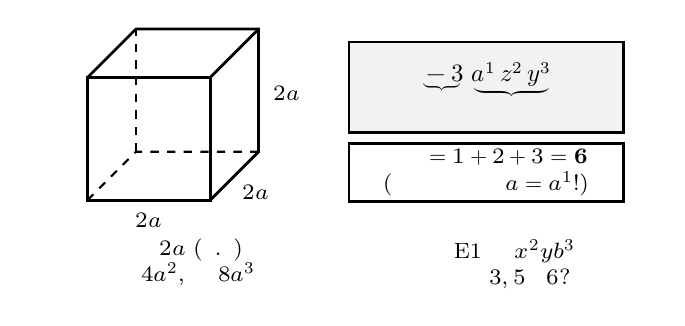
\begin{tikzpicture}[scale=0.82, every node/.style={font=\footnotesize, text=black}]
  % ឆ្វេង៖ គូបទ្រនុង 2a (ទំ.៥១)
  \begin{scope}[shift={(0,0)}]
    \draw[black, line width=1.0pt] (0.20,0.20) rectangle (2.10,2.10);
    \draw[black, line width=1.0pt] (2.10,0.20) -- (2.85,0.95) -- (2.85,2.85) -- (0.95,2.85) -- (0.20,2.10);
    \draw[black, line width=1.0pt] (2.10,2.10) -- (2.85,2.85);
    \draw[black, line width=0.75pt, dashed] (0.20,0.20) -- (0.95,0.95) -- (2.85,0.95);
    \draw[black, line width=0.75pt, dashed] (0.95,0.95) -- (0.95,2.85);
    \node[below=1pt] at (1.15,0.20) {$2a$};
    \node[below right=-1pt] at (2.48,0.56) {$2a$};
    \node[right=2pt] at (2.85,1.85) {$2a$};
    \node[anchor=north, text width=3.45cm, align=center] at (1.52,-0.25) {គូបទ្រនុង $2a$ (ទំ.៥១)៖\\ផ្ទៃមុខ $4a^2$, មាឌ $8a^3$};
  \end{scope}
  % ស្ដាំ៖ រចនាសម្ព័ន្ធធាតុផ្សំនៃឯកធា x^2 y^1 b^3
  \begin{scope}[shift={(4.15,0)}]
    \draw[black, line width=0.95pt, fill=gray!10] (0.10,1.25) rectangle (4.35,2.65);
    \node[font=\small] at (2.22,1.95) {$\underbrace{-3}_{\text{មេគុណ}}\,\underbrace{a^{1}\,z^{2}\,y^{3}}_{\text{ផ្នែកអថេរ}}$};
    \draw[black, line width=0.85pt] (0.10,0.18) rectangle (4.35,1.08);
    \node[align=center] at (2.22,0.63) {ដឺក្រេ $= 1 + 2 + 3 = \mathbf{6}$\\(កុំភ្លេចនិទស្សន្ត $a = a^1$!)};
    \node[anchor=north, text width=4.10cm, align=center] at (2.22,-0.25) {បេសកកម្ម E1៖ តើ $x^2yb^3$\\មានដឺក្រេស្មើ $3, 5$ ឬ $6$?};
  \end{scope}
\end{tikzpicture}}

% ២. E3 Explain: ដ្យាក្រាមប្រៀបធៀប «ឯកធា» vs «មិនមែនឯកធា» និង «ឯកធាដូចគ្នា»
\newcommand{\figAnatomyALGOne}{%
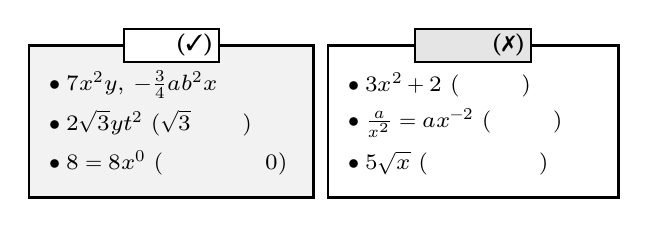
\begin{tikzpicture}[scale=0.73, every node/.style={font=\footnotesize, text=black}]
  % ប្រអប់ឆ្វេង៖ ជាឯកធា
  \draw[black, line width=1.0pt, fill=gray!10] (0,0.15) rectangle (4.95,2.80);
  \node[fill=white, draw=black, line width=0.7pt, inner sep=2pt] at (2.475,2.80) {\textbf{ជាឯកធា (\ding{51})}};
  \node[anchor=west] at (0.18,2.12) {$\bullet\; 7x^2y,\; -\frac{3}{4}ab^2x$};
  \node[anchor=west] at (0.18,1.45) {$\bullet\; 2\sqrt{3}yt^2$ ($\sqrt{3}$ ជាមេគុណ)};
  \node[anchor=west] at (0.18,0.75) {$\bullet\; 8 = 8x^0$ (ចំនួនថេរ ដឺក្រេ $0$)};

  % ប្រអប់ស្ដាំ៖ មិនមែនឯកធា
  \draw[black, line width=1.0pt] (5.20,0.15) rectangle (10.25,2.80);
  \node[fill=gray!20, draw=black, line width=0.7pt, inner sep=2pt] at (7.725,2.80) {\textbf{មិនមែនឯកធា (\ding{55})}};
  \node[anchor=west] at (5.38,2.12) {$\bullet\; 3x^2 + 2$ (មានវិធីបូក)};
  \node[anchor=west] at (5.38,1.45) {$\bullet\; \frac{a}{x^2} = ax^{-2}$ (ចែកនឹងអថេរ)};
  \node[anchor=west] at (5.38,0.75) {$\bullet\; 5\sqrt{x}$ (អថេរក្រោមរ៉ាឌីកាល់)};
\end{tikzpicture}}

\begin{document}
\fontsize{10pt}{15.2pt}\selectfont

% -------------------- ក្បាលកិច្ចតែងការ (Header) --------------------
\begin{center}
  {\muol\fontsize{11pt}{16pt}\selectfont ព្រះរាជាណាចក្រកម្ពុជា}\\[2pt]
  {\muol\fontsize{10pt}{15pt}\selectfont ជាតិ សាសនា ព្រះមហាក្សត្រ}\\[1pt]
  \khmflourish
\end{center}

\vspace{-28pt}
{\muol\fontsize{9.5pt}{12.5pt}\selectfont
មន្ទីរអប់រំ យុវជន និងកីឡា ខេត្តកំពង់ធំ\\
ការិយាល័យអប់រំ យុវជន និងកីឡា ស្រុកកំពង់ស្វាយ\\
អនុវិទ្យាល័យព្រះក្រសាំង}

\vspace{1pt}
\begin{center}
  {\muol\fontsize{10pt}{14pt}\selectfont កិច្ចតែងការបង្រៀន}
\end{center}
\vspace{0pt}

% -------------------- ព័ត៌មានទូទៅ (Metadata) --------------------
{\renewcommand{\arraystretch}{0.95}
\hspace*{4.05cm}%
\begin{tabular}{@{}l l l@{}}
  - \hspace{0.35cm} មុខវិជ្ជា & : & គណិតវិទ្យា ថ្នាក់ទី៨ \\
  - \hspace{0.35cm} ចំណងជើងមេរៀន & : & មេរៀនទី៥ កន្សោមពីជគណិត \\
  - \hspace{0.35cm} ចំណងជើងរង & : & ១.១--១.៣ សញ្ញាណឯកធា ឯកធាដូចគ្នា និងដឺក្រេនៃឯកធា (ទំ.៥១--៥៣) \\
  - \hspace{0.35cm} រយៈពេល & : & ១ ម៉ោងសិក្សា (៥០ នាទី) \\
  - \hspace{0.35cm} បង្រៀនដោយ & : & ហុក ប៊ុនថែន \\
  - \hspace{0.35cm} កាលបរិច្ឆេទ & : & ថ្ងៃសុក្រ ១០រោច ខែកត្តិក ព.ស.២៥៧០ (៤ ធ្នូ ២០២៦) \\
\end{tabular}
}

\vspace{1pt}

% -------------------- I. វត្ថុបំណង --------------------
\textbf{I.} {\muol វត្ថុបំណង}\\[1pt]
\hspace*{0.55cm}%
\begin{tabular}{@{}l l L{14.2cm}@{}}
  \wcirc \hspace{0.25cm} វិជ្ជាសម្បទា & : & សិស្សប្រាប់បានត្រឹមត្រូវនូវនិយមន័យ \textbf{កន្សោមពីជគណិត} \textbf{ឯកធា} (មានតែប្រមាណវិធីគុណ និងស្វ័យគុណដែលមាននិទស្សន្តជាចំនួនគត់វិជ្ជមាន ឬសូន្យ) \textbf{មេគុណ} \textbf{ផ្នែកអថេរ} \textbf{ឯកធាដូចគ្នា} (ផ្នែកអថេរដូចគ្នាបេះបិទ) និង \textbf{ដឺក្រេនៃឯកធា} (ផលបូកនិទស្សន្តនៃអថេរទាំងអស់) តាមសៀវភៅគោល ទំ.៥១--៥៣ ។ \\
  \wcirc \hspace{0.25cm} បំណិនសម្បទា & : & សិស្សញែកដាច់រវាងឯកធា និងកន្សោមមិនមែនឯកធា (មានបូក/ដក ឬចែកនឹងអថេរ) ជ្រើសរើសគូឯកធាដូចគ្នា និងគណនាដឺក្រេនៃឯកធាច្រើនអថេរដោយមិនភ្លេចនិទស្សន្តលាក់មុខ $1$ លើសន្លឹកកិច្ចការស-ខ្មៅបានត្រឹមត្រូវ ។ \\
  \wcirc \hspace{0.25cm} ចរិយាសម្បទា & : & សិស្សមានទម្លាប់ពិនិត្យរចនាសម្ព័ន្ធនិមិត្តសញ្ញាពីជគណិតយ៉ាងហ្មត់ចត់ មិនវិនិច្ឆ័យដោយមើលត្រួសៗ និងសហការពិភាក្សាដៃគូប្រកបដោយទំនុកចិត្ត ។ \\
\end{tabular}

\vspace{1pt}

% -------------------- II. សម្ភារៈឧបទេស --------------------
\textbf{II.} {\muol សម្ភារៈឧបទេស}\\[1pt]
\hspace*{0.55cm}$\bullet$ \hspace{0.35cm} សៀវភៅសិក្សាគោលគណិតវិទ្យាថ្នាក់ទី៨ (ទំ.៥១--៥៣ និងទំ.៧២) ក្ដារខៀន ដីស បន្ទាត់ និងសន្លឹកកិច្ចការសិស្សស-ខ្មៅ (\en{Worksheet\_ALG51} ចំនួន ២ ទំព័រ \en{A4} ដោយគ្មានស្លាយ \en{LCD}) ។

\vspace{1pt}

% -------------------- III. វិធីសាស្រ្តបង្រៀន --------------------
\textbf{III.} {\muol វិធីសាស្រ្តបង្រៀន}\\[1pt]
\hspace*{0.55cm}$\bullet$ \hspace{0.35cm} គោលវិធីសិស្សមជ្ឈមណ្ឌលតាមគំរូ \en{5Es} រួមបញ្ចូល \textbf{តារាងញែកឧទាហរណ៍ និងមិនមែនឧទាហរណ៍តាមគំរូ \en{Frayer}} (\en{Moru \& Mathunya, 2022}) និង \textbf{ការវិភាគអត្តសញ្ញាណផ្នែកអថេរ និងនិទស្សន្តលាក់មុខ} (\en{Aydin-G\"u\c{c} \& Ayg\"un, 2021}) ។

\vspace{2pt}

% -------------------- IV. ដំណើរការបង្រៀន --------------------
\textbf{IV.} {\muol ដំណើរការបង្រៀន}\\[-6pt]

{\renewcommand{\arraystretch}{1.15}
\begin{longtable}{|L{5.50cm}|L{7.90cm}|L{4.80cm}|}
\hline
\multicolumn{1}{|c|}{\cellcolor{headgray}\muol សកម្មភាពគ្រូ} &
\multicolumn{1}{c|}{\cellcolor{headgray}\muol ខ្លឹមសារមេរៀន} &
\multicolumn{1}{c|}{\cellcolor{headgray}\muol សកម្មភាពសិស្ស} \\[2pt]
\hline
\endfirsthead

\hline
\multicolumn{1}{|c|}{\cellcolor{headgray}\muol សកម្មភាពគ្រូ} &
\multicolumn{1}{c|}{\cellcolor{headgray}\muol ខ្លឹមសារមេរៀន} &
\multicolumn{1}{c|}{\cellcolor{headgray}\muol សកម្មភាពសិស្ស} \\[2pt]
\hline
\endhead

\hline
\endfoot

% ==================== ជំហានទី១ (2min) ====================
\stepheader{ជំហានទី១ ៖ រដ្ឋបាលថ្នាក់ (២ នាទី)}
$\bullet$ ពិនិត្យអវត្តមាន សណ្ដាប់ធ្នាប់ អនាម័យ និងការត្រៀមសៀវភៅគោល \par\vspace{1pt}
$\bullet$ ចែកសន្លឹកកិច្ចការស-ខ្មៅ \en{Worksheet\_ALG51} (១ សន្លឹកសងខាងក្នុងម្នាក់)
&
$\bullet$ វត្តមានសិស្ស ឯកសណ្ឋាន និងសណ្ដាប់ធ្នាប់ថ្នាក់រៀន \par
$\bullet$ សន្លឹកកិច្ចការសិស្ស \en{Worksheet\_ALG51} (ទំព័រ ១--២) រួចរាល់លើតុ
&
$\circ$ ប្រធានថ្នាក់រាយការណ៍អវត្តមាន \par
$\circ$ សរសេរឈ្មោះលើសន្លឹកកិច្ចការ \\
\hline

% ==================== ជំហានទី២ (9min) ====================
\stepheader{ជំហានទី២ ៖ កែកិច្ចការផ្ទះ រំលឹកមេរៀនចាស់ និងភ្ជាប់បញ្ហាថ្មី (៩ នាទី)}
\ditem \textbf{កែកិច្ចការផ្ទះ ($\le 3\unit{min}$)៖} \par
$\bullet$ ហៅសិស្ស ១ រូបឡើងកែលំហាត់ល្បឿនមធ្យមពីមេរៀនទី៤ (ទំ.៥០) លើក្ដារខៀន
&
\textbf{កំណែកិច្ចការផ្ទះ (មេរៀនទី៤ ទំ.៥០)៖} \par
រថយន្តមួយបើកបរបានចម្ងាយ $d = 120\unit{km}$ ក្នុងរយៈពេល $t = 2\unit{h}\;30\unit{mn} = 2.5\unit{h}$ ។ ល្បឿនមធ្យមគឺ៖
\[ v = \frac{d}{t} = \frac{120}{2.5} = \mathbf{48\unit{km/h}} \]
&
$\circ$ ផ្ទៀងផ្ទាត់ការបំប្លែងម៉ោង $2\unit{h}\;30\unit{mn} = 2.5\unit{h}$ និងកែសម្រួលចម្លើយ \\[3pt]

\ditem \textbf{រំលឹកមេរៀនចាស់ ($3\unit{min}$)៖} \par
$\bullet$ សួររំលឹកពីនិយមន័យស្វ័យគុណ $a^n$, តម្លៃ $a^1$, $a^0$ ($a\ne 0$) និងផ្ទៃ-មាឌគូប
&
\textbf{សំណួររំលឹកមូលដ្ឋានគ្រឹះស្វ័យគុណ (មេរៀនទី២)៖} \par
១) $x^1 = x$ និងចំពោះ $x \ne 0 \implies x^0 = 1$ (ឧ. $8x^0 = 8\times 1 = 8$) ។ \par
២) $(2a)^2 = 2^2 a^2 = 4a^2$ និង $(2a)^3 = 2^3 a^3 = 8a^3$ ។
&
$\circ$ ឆ្លើយរំលឹកលក្ខណៈស្វ័យគុណនៃផលគុណ និងតម្លៃ $x^0 = 1$ \\[3pt]

\fiveE{E1 - Engage} \timenote{(3 នាទី)} \par\vspace{1pt}
$\bullet$ គូសរូបគូបទ្រនុង $2a$ (ទំ.៥១) លើក្ដារខៀន រួចឱ្យសិស្សគូសធីកការទស្សន៍ទាយដឺក្រេនៃ $x^2yb^3$ ក្នុងផ្នែកទី១ នៃសន្លឹកកិច្ចការ
&
\textbf{ស្ថានភាពភ្ជាប់បញ្ហា៖ គូបទ្រនុង $2a$ និងអាថ៌កំបាំងដឺក្រេ $x^2yb^3$} \par
គូបមួយមានទ្រនុងប្រវែង $2a$ ៖ ផ្ទៃមុខខាងនីមួយៗស្មើ $4a^2$ និងមាឌស្មើ $8a^3$ ។ កន្សោម $2a, 4a^2, 8a^3$ និង $x^2yb^3$ សុទ្ធតែជា \textbf{ឯកធា} ។ \par
\hspace*{0.3em}– \textbf{សំណួរបេសកកម្ម៖} «ចំពោះឯកធា $x^2yb^3$ តើវាមានដឺក្រេស្មើ $3$ (យកនិទស្សន្តខ្ពស់បំផុត) ស្មើ $5$ ($2+3$) ឬស្មើ $6$ ($2+1+3$)?»
&
$\circ$ សង្កេតរង្វាស់ $2a, 4a^2, 8a^3$ \par
$\circ$ គូសធីកការទស្សន៍ទាយមុនរៀន ($3, 5$ ឬ $6$) ក្នុងប្រអប់ផ្នែកទី១ \\[3pt]

& \cfig{\figEngageALGOne} & \\
\hline

% ==================== ជំហានទី៣ (17min) ====================
\stepheader{ជំហានទី៣ ៖ មេរៀនថ្មី — សញ្ញាណឯកធា ឯកធាដូចគ្នា និងដឺក្រេនៃឯកធា (១៧ នាទី)}
\fiveE{E2 - Explore} \timenote{(11 នាទី)} \par\vspace{1pt}
\ditem \textbf{សកម្មភាពទី១៖ តារាងញែកឯកធា និងមិនមែនឯកធា ($5.5\unit{min}$)៖} \par
$\bullet$ ឱ្យសិស្សធ្វើការជាដៃគូលើ \textbf{ផ្នែកទី២ (ក)} នៃ \en{Worksheet\_ALG51} ដើម្បីញែកកន្សោមទាំង ៨ តាមប្រភេទប្រមាណវិធី
&
\textbf{ការរុករកទី១ (តាមលំនាំសៀវភៅគោល ទំ.៥១--៥២)៖} \par
ពិនិត្យកន្សោមទាំង ៨៖ $\frac{1}{5}x^2y,\; 3x^2+2,\; 25,\; -\frac{2}{3}a^4bc^2,\; \frac{a}{x^2},\; 2\sqrt{3}yt^2,\; zx^2a^3b^4,\; 5\sqrt{x}$ ៖ \par
$\bullet$ \textbf{ជាឯកធា៖} $\frac{1}{5}x^2y,\; 25 (=25x^0),\; -\frac{2}{3}a^4bc^2,\; 2\sqrt{3}yt^2,\; zx^2a^3b^4$ (មានតែគុណ និងស្វ័យគុណគត់វិជ្ជមាន ឬសូន្យ) ។ \par
$\bullet$ \textbf{មិនមែនឯកធា៖} $3x^2+2$ (មានបូក), $\frac{a}{x^2}=ax^{-2}$ (ចែកនឹងអថេរ/និទស្សន្តអវិជ្ជមាន), $5\sqrt{x}$ (អថេរជាប់រ៉ាឌីកាល់) ។
&
$\circ$ ពិភាក្សាដៃគូបំពេញតារាងញែកកន្សោម \par
$\circ$ រកឃើញថាចំនួនថេរ $25 = 25x^0$ ក៏ជាឯកធាដែរ \\[3pt]

\ditem \textbf{សកម្មភាពទី២៖ អន្ទាក់ឯកធាដូចគ្នា និងនិទស្សន្តលាក់មុខ $1$ ($5.5\unit{min}$)៖} \par
$\bullet$ ឱ្យដៃគូបន្តបំពេញ \textbf{ផ្នែកទី២ (ខ--គ)}៖ ប្រៀបធៀប $-2x^2y$ នឹង $2xy^2$ និងគណនាដឺក្រេដោយសរសេរ $y = y^1$
&
\textbf{ការរុករកទី២ (ឯកធាដូចគ្នា និងដឺក្រេ ទំ.៥២--៥៣)៖} \par
$\bullet$ \textbf{អន្ទាក់ឯកធាដូចគ្នា៖} $-2x^2y$ (មាន $x^2y^1$) និង $2xy^2$ (មាន $x^1y^2$) \textbf{មិនមែន} ជាឯកធាដូចគ្នាទេ ព្រោះនិទស្សន្តលើ $x$ និង $y$ ខុសគ្នា! ឯកធាដូចគ្នាត្រូវមានផ្នែកអថេរដូចគ្នាបេះបិទ (ឧ. $\frac{1}{2}xy$ និង $xy$) ។ \par
$\bullet$ \textbf{អន្ទាក់ដឺក្រេ៖} ចំពោះ $x^2yb^3 = x^2 y^{\mathbf{1}} b^3$ អថេរ $y$ មាននិទស្សន្តលាក់មុខស្មើ $1$ ដូច្នេះដឺក្រេគឺ $2 + 1 + 3 = \mathbf{6}$ (មិនមែន $5$ ឬ $3$ ទេ!) ។
&
$\circ$ ប្រៀបធៀបផ្នែកអថេរ $x^2y$ ទល់នឹង $xy^2$ \par
$\circ$ សរសេរនិទស្សន្តលាក់មុខ $1$ លើអថេរគ្មានលេខពីលើ រួចបូកនិទស្សន្តទាំងអស់ \\[3pt]

\fiveE{E3 - Explain} \timenote{(6 នាទី)} \par\vspace{1pt}
$\bullet$ ហៅតំណាងដៃគូឡើងបង្ហាញ រួចគ្រូសង្ខេបនិយមន័យទាំង ៣ និងធនាគារហេតុផល \cnum{1}--\cnum{5} លើក្ដារខៀន
&
\textbf{មេរៀនទី៥៖ កន្សោមពីជគណិត — ១. ឯកធា (ទំ.៥១--៥៣)} \par
$\bullet$ \textbf{១.១ សញ្ញាណឯកធា (\cnum{1})៖} \textbf{ឯកធា} គឺជាកន្សោមពីជគណិតដែលមានតែប្រមាណវិធីគុណ និងស្វ័យគុណដែលនិទស្សន្តជាចំនួនគត់វិជ្ជមាន ឬសូន្យ ។ ឧ. ចំពោះ $7x^2y$ មាន $7$ ជា \textbf{មេគុណ} និង $x, y$ ជា \textbf{អថេរ} ($x^2y$ ជាផ្នែកអថេរ) ។ \par
$\bullet$ \textbf{សម្គាល់ (\cnum{2})៖} ចំនួនថេរមិនសូន្យ (ឧ. $8 = 8x^0$) ក៏ជាឯកធាដែរ និងមានដឺក្រេស្មើ $0$ ។
&
$\circ$ ឡើងបកស្រាយលទ្ធផលរុករក \par
$\circ$ កត់ត្រានិយមន័យចូលក្នុងប្រអប់ផ្នែកទី៣ នៃសន្លឹកកិច្ចការ \\[3pt]

$\bullet$ សង្កត់ធ្ងន់និយមន័យឯកធាដូចគ្នា (\cnum{3}) និងដឺក្រេនៃឯកធា (\cnum{4}--\cnum{5})
&
$\bullet$ \textbf{១.២ ឯកធាដូចគ្នា (\cnum{3})៖} គឺជាឯកធាដែលមាន \textbf{ផ្នែកអថេរដូចគ្នា} (អថេរដូចគ្នា និងនិទស្សន្តតាមអថេរនីមួយៗស្មើគ្នា ទោះបីមេគុណខុសគ្នាក៏ដោយ) ។ \par
$\bullet$ \textbf{១.៣ ដឺក្រេនៃឯកធា (\cnum{4})៖} គឺជា \textbf{ផលបូកនិទស្សន្តរបស់អថេរនីមួយៗ} នៃឯកធា ។ (\cnum{5} អថេរដែលគ្មានសរសេរនិទស្សន្ត គឺមាននិទស្សន្តស្មើ $1$ ៖ $x = x^1$) ។
&
$\circ$ កត់ចំណាំច្បាប់និទស្សន្តលាក់មុខ $x = x^1$ និងដឺក្រេចំនួនថេរស្មើ $0$ \\[3pt]

& \cfig{\figAnatomyALGOne} & \\
\hline

% ==================== ជំហានទី៤ (20min) ====================
\stepheader{ជំហានទី៤ ៖ ពង្រីកចំណេះដឹង និងវាយតម្លៃលទ្ធផលសិក្សា (២០ នាទី)}
\fiveE{E4 - Elaborate} \timenote{(10 នាទី)} \par\vspace{1pt}
\ditem \textbf{លំហាត់គំរូទី១ និងទី២ (ទំ.៥២, $4.5\unit{min}$)៖} \par
$\bullet$ ដឹកនាំសិស្សវិភាគលំហាត់គំរូទំ.៥២ លើក្ដារខៀន និងបំពេញក្នុង \textbf{ផ្នែកទី៤} នៃសន្លឹកកិច្ចការ
&
\textbf{លំហាត់គំរូទី១ និងទី២ (សៀវភៅគោល ទំ.៥២)៖} \par
១) ឯកធា $-\frac{3}{4}ab^2x$ មាន \textbf{មេគុណ} $-\frac{3}{4}$ (ភ្ជាប់ទាំងសញ្ញាដក!), \textbf{អថេរ} $a, b, x$ និង \textbf{ផ្នែកអថេរ} $ab^2x$ ។ \par
២) ក្នុងចំណោម $5x^2yz^3,\; \frac{7}{2}x^2cy^3,\; 5a^2bc^3,\; \frac{1}{2}x^2yz^3$ គេបាន \textbf{$5x^2yz^3$ និង $\frac{1}{2}x^2yz^3$} ជា \textbf{ឯកធាដូចគ្នា} ព្រោះមានផ្នែកអថេរ $x^2yz^3$ ដូចគ្នា (\cnum{3}) ។
&
$\circ$ គូសរង្វង់មេគុណទាំងសញ្ញា $-\frac{3}{4}$ និងគូសបន្ទាត់ក្រោមផ្នែកអថេររួម $x^2yz^3$ \\[3pt]

\ditem \textbf{លំហាត់គំរូទី៣ (តារាងដឺក្រេ ទំ.៥២--៥៣) និងឆ្លុះបញ្ចាំង ($5.5\unit{min}$)៖} \par
$\bullet$ ឱ្យសិស្សបំពេញតារាងដឺក្រេ ៤ ជួរ (ទំ.៥៣) រួចចោទសំណួរឆ្លុះបញ្ចាំងលើរ៉ាឌីកាល់
&
\textbf{លំហាត់គំរូទី៣ (ទំ.៥២--៥៣)៖ កំណត់អថេរ និងដឺក្រេនៃឯកធា} \par
\vspace{2pt}
{\footnotesize\renewcommand{\arraystretch}{1.15}
\begin{tabular}{|L{2.2cm}|L{2.0cm}|L{3.0cm}|}
\hline
\cellcolor{headgray}\textbf{ឯកធា} & \cellcolor{headgray}\textbf{អថេរ} & \cellcolor{headgray}\textbf{ដឺក្រេ (ផលបូកនិទស្សន្ត)} \\[2pt]
\hline
$x^2yb^3$ & $x, y, b$ & $2 + 1 + 3 = \mathbf{6}$ \\
\hline
$\frac{3}{4}a^2bc$ & $a, b, c$ & $2 + 1 + 1 = \mathbf{4}$ \\
\hline
$x^3y^2$ & $x, y$ & $3 + 2 = \mathbf{5}$ \\
\hline
$-3az^2y^3$ & $a, z, y$ & $1 + 2 + 3 = \mathbf{6}$ \\
\hline
\end{tabular}} \par\vspace{2pt}
$\bullet$ \textbf{សំណួរឆ្លុះបញ្ចាំង៖} $\sqrt{5}ax^2$ ជាឯកធា (ដឺក្រេ $1+2=3$) ព្រោះរ៉ាឌីកាល់នៅលើមេគុណ $\sqrt{5}$ មិនមែនលើអថេរទេ!
&
$\circ$ បំពេញតារាងដឺក្រេទាំង ៤ ជួរ \par
$\circ$ ពន្យល់ភាពខុសគ្នារវាង $\sqrt{5}ax^2$ (ជាឯកធា) និង $5\sqrt{x}$ (មិនមែនឯកធា) \\[3pt]

\fiveE{E5 - Evaluate} \timenote{(10 នាទី)} \par\vspace{1pt}
\ditem \textbf{អនុវត្ត «ប្រតិបត្តិ» (ទំ.៥២--៥៣, $6.5\unit{min}$)៖} \par
$\bullet$ ឱ្យសិស្សធ្វើលំហាត់ \textbf{ប្រតិបត្តិ} (ទំ.៥២ និងទំ.៥៣) ដោយខ្លួនឯងក្នុងផ្នែកទី៥ នៃសន្លឹកកិច្ចការ រួចប្ដូរសន្លឹកកិច្ចការផ្ទៀងជាដៃគូ
&
\textbf{ចម្លើយលំហាត់ «ប្រតិបត្តិ» (សៀវភៅគោល ទំ.៥២--៥៣)៖} \par
១) \textbf{ទំ.៥២៖} ចំពោះ $2\sqrt{3}yt^2$ មានមេគុណ $2\sqrt{3}$ និងអថេរ $y, t$ ។ ក្នុងចំណោម $\frac{1}{2}xy, -2x^2y, ay, 3ax, 2xy^2, xy$ គូឯកធាដូចគ្នាគឺ \textbf{$\frac{1}{2}xy$ និង $xy$} (ព្រោះ $xy = 1xy$) ។ \par
២) \textbf{ទំ.៥៣ (កំណត់អថេរ និងដឺក្រេ)៖} \par
\hspace*{0.3em}– ក) $\frac{1}{2}xyz \to x,y,z$ (ដឺក្រេ $\mathbf{3}$) \quad;\quad ខ) $8x^3yz^2 \to x,y,z$ (ដឺក្រេ $\mathbf{6}$) \par
\hspace*{0.3em}– គ) $14 \to$ គ្មានអថេរ (ដឺក្រេ $\mathbf{0}$) \quad;\quad ឃ) $21ab^4c \to a,b,c$ (ដឺក្រេ $\mathbf{6}$) \par
\hspace*{0.3em}– ង) $3x^2y^3z^4 \to x,y,z$ (ដឺក្រេ $\mathbf{9}$) \quad;\quad ច) $axyz \to a,x,y,z$ (ដឺក្រេ $\mathbf{4}$) ។
&
$\circ$ គណនាដោយខ្លួនឯង រួចប្ដូរសន្លឹកកិច្ចការផ្ទៀងផ្ទាត់ជាមួយដៃគូ (\en{Pause-Review}) \\[3pt]

\ditem \textbf{បិទបេសកកម្ម E1 និងតេស្តរហ័ស \en{Exit Check} ($3.5\unit{min}$)៖} \par
$\bullet$ សួរបិទបេសកកម្ម $x^2yb^3$ និងឱ្យសិស្សជ្រើសរើស \en{A--D} លើសន្លឹកកិច្ចការ
&
$\bullet$ \textbf{បិទបេសកកម្ម E1៖} ឯកធា $x^2yb^3 = x^2y^1b^3$ មានដឺក្រេ $2 + 1 + 3 = \mathbf{6}$ ។ \par
$\bullet$ \textbf{Exit Check៖} តើឯកធា $-\frac{5}{7}m^3np^4$ មានមេគុណ និងដឺក្រេស្មើប៉ុន្មាន? \par
\en{A.} មេគុណ $\frac{5}{7}$, ដឺក្រេ $7$ \quad \en{B.} មេគុណ $-\frac{5}{7}$, ដឺក្រេ $7$ \par
\graybox{\enbf{C.} មេគុណ $-\frac{5}{7}$, ដឺក្រេ $8$ \ding{51}} \quad \en{D.} មេគុណ $-\frac{5}{7}$, ដឺក្រេ $12$
&
$\circ$ បូកនិទស្សន្ត $3 + 1 + 4 = 8$ ជាមួយមេគុណ $-\frac{5}{7}$ រួចគូសរង្វង់ជម្រើស \textbf{C} \\
\hline

% ==================== ជំហានទី៥ (<=2min) ====================
\stepheader{ជំហានទី៥ ៖ កិច្ចការផ្ទះ និងបណ្ដាំផ្ញើ ($\le$ ២ នាទី)}
$\bullet$ កត់ត្រាកិច្ចការផ្ទះលើក្ដារខៀន (មានបោះពុម្ពស្រាប់នៅផ្នែកទី៦ នៃសន្លឹកកិច្ចការទំព័រទី២) \par
$\bullet$ រំលឹកគន្លឹះសង្កេតចំពោះ $\frac{x^3}{3} = \frac{1}{3}x^3$ និង $x(x+y)$ មុនធ្វើកិច្ចការផ្ទះ
&
\textbf{កិច្ចការផ្ទះ (សៀវភៅសិក្សាគោល ទំ.៧២)៖} \par
១. \textbf{លំហាត់ទី១ (ទំ.៧២)៖} តើកន្សោមខាងក្រោមមួយណាជាឯកធា? បើជាឯកធា ចូរប្រាប់មេគុណ និងដឺក្រេរបស់វា៖ $\frac{x^3}{3},\; \sqrt{5}ax^2,\; \frac{7xy^2}{3},\; x+2y,\; \frac{a}{x^2},\; x(x+y)$ ។ \par
\hspace*{0.3em}\textit{(គន្លឹះ៖ ចែកនឹងចំនួនថេរ $\frac{x^3}{3} = \frac{1}{3}x^3$ ជាឯកធា ចំណែក $x(x+y) = x^2+xy$ មានបូក)} ។ \par
២. សរសេរឯកធាពីរដែលជា \textbf{ឯកធាដូចគ្នា} មានអថេរ $x, y$ និងមានដឺក្រេស្មើ $5$ (ឧទាហរណ៍ទម្រង់ $kx^2y^3$ ឬ $kx^4y$) ។
&
$\circ$ កត់ត្រាកិច្ចការផ្ទះ និងគន្លឹះសង្កេត \par
$\circ$ ទុកដាក់សន្លឹកកិច្ចការក្នុងសឺមីគណិតវិទ្យាឱ្យមានរបៀប \\[3pt]

$\bullet$ ណែនាំឱ្យអានចំណុច ១.៤--១.៦ ជាមុនសម្រាប់ម៉ោងក្រោយ
&
$\bullet$ \textbf{អានជាមុន៖} ចំណុច \textbf{១.៤ ដល់ ១.៦ ប្រមាណវិធីបូក ដក គុណ និងចែកឯកធា} (សៀវភៅគោល ទំព័រ ៥៣--៥៦) និងសង្កេតភាពខុសគ្នារវាងការបូកឯកធាដូចគ្នា និងការគុណឯកធា ។
&
$\circ$ ទទួលបណ្ដាំផ្ញើ និងជម្រាបលាគ្រូ \\

\end{longtable}
}

\vspace{6pt}

% -------------------- ហត្ថលេខា (Signature Block) --------------------
\begin{flushright}
\begin{minipage}{9.6cm}
\centering
ថ្ងៃសុក្រ ១០រោច ខែកត្តិក ឆ្នាំមមី អដ្ឋស័ក ពុទ្ធសករាជ ២៥៧០\\[2pt]
ព្រះក្រសាំង, ថ្ងៃទី៤ ខែធ្នូ ឆ្នាំ២០២៦\\[4pt]
{\muol គ្រូបង្រៀន}\\[32pt]
\hfill{\muol ហុក ប៊ុនថែន}\hspace*{1.4cm}
\end{minipage}
\end{flushright}

\end{document}
